
In this chapter, the methodology for the experiments for this study
is described and elaborated. The experiments will be conducted to evaluate the performance of
\textit{reUpNix} as a host
operating system for \textit{Azure IoT Edge} and to investigate the efficiency
of its update mechanism. There will be an emphasis on the size of the \ac{OS}
image, the size of the updates, the time to recover, and the efficiency of
updating container images.

\section{Image Size}
\label{sec:image-size}
Reducing the image size of an operating system is crucial for \ac{IoT} devices
with low bandwidth or limited storage capacity, regardless of which update
methodology is used. In environments where network connectivity is limited or expensive,
smaller image sizes result in faster and more efficient updates with a traditional
A/B partition schema.

By reducing the number of packages and components that are installed on the
system or removing unused software entirely, the number of files that need to
be transmitted during an update will also be reduced. Therefore,
a minimal operating system image that is significantly smaller
than Microsoft's recommended \textit{Ubuntu 22.04} needs to be created, while
still being able to run the
\textit{Azure IoT Edge} runtime and the required software. To investigate if using
a different update methodology is more efficient than using an A/B partition schema,
this image must also feature the update mechanism of \textit{reUpNix}.

However, it must be considered that\textit{Azure Iot Edge} is not officially
supported on \textit{NixOS}
by Microsoft and there is no \textit{Nix} package available. Therefore, a \textit{Nix} package
for \textit{Azure IoT Edge} and all of its dependencies from the publicly available source code
needs to be created. This is a crucial step, since
without a working \textit{Azure IoT Edge} runtime, there cannot be drawn any meaningful
conclusions for updating \ac{IIoT} devices using \textit{Azure IoT}.

To create the \textit{Nix} packages, the dependencies of
\textit{Azure IoT Edge} and how to package them needs to be understood.
As it can be seen in figure
\ref{fig:dependency-tree}, \textit{Azure IoT Edge} runtime has a tree of dependencies,
many of which are common to \textit{Linux} systems, which means that the over
80,000\footnote{Current number retrieved from the Nix search page: https://search.nixos.org/packages}
already existing \textit{Nix} packages can be utilized to meet those dependencies.

\begin{figure}[H]
    \centering
    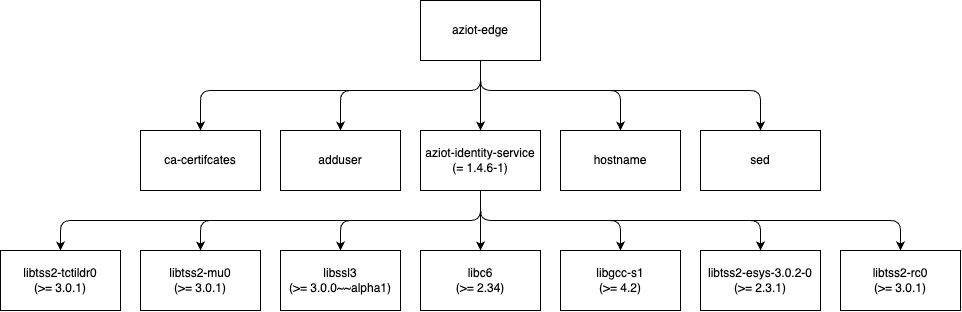
\includegraphics[width=\textwidth]{fig/dependecy-tree.drawio.png}
    \caption{Azure IoT Edge Dependency Tree}
    \label{fig:dependency-tree}
\end{figure}

\noindent
Once a minimal operating system image using \textit{reUpNix} has been created, the size of the image
needs to be measured. Then the measurements for
\textit{Ubuntu 22.04}, \textit{Yocto Kirkstone}, and \textit{NixOS} have to be conducted, such that
it is possible to compare the operating systems and draw a conclusion.

\subsection{Hypothesis}
Since \textit{reUpNix} has already shown to be able to reduce the size of the
operating system image \cite{gollenstede:23:lctes}, it is hypothesized that the
image size of \textit{reUpNix} including the \textit{Azure IoT Edge} runtime
will also be significantly smaller than the image size of \textit{NixOS},
\textit{Ubuntu 22.04}, and \textit{Yocto Kirkstone}.


\section{Update size}
\label{sec:update-size}
When updating the operating system with an A/B partition schema, the entire
image needs to be downloaded and written to a secondary partition. In this
\ac{OTA} scenario, the size of the operating system image is critical, as it has been
already elaborated in chapter \ref{sec:image-size}.
However, if a different methodology than an A/B partition schema is being adapted
for updating the operating system, the update size can potentially be reduced
drastically.

It has to be established, if using \textit{reUpNix}'s differential updates as the
update mechanism for an \ac{IIoT} device with \textit{Azure IoT Edge}
will result in a smaller update size in comparison to using an A/B partition schema with
\textit{Ubuntu 22.04} and \textit{Yocto Kirkstone}. To do so, an update for a \textit{reUpNix} system,
in which the majority of software packages installed is being upgraded, needs to be created, so that it is comparable
to a distribution upgrade of \textit{Ubuntu 22.04} and \textit{Yocto Kirkstone}.

Importantly, the created updates, regardless for which \ac{OS}, must all be
able to be installed using the \textit{Azure IoT Update Service} and respective
\textit{Azure IoT Update Agent}. Since the \textit{Azure IoT Update Agent} is
not officially supported on \textit{NixOS}, a \textit{Nix} package
for the \textit{Azure IoT Update Agent} and all of its dependencies needs to be created.

\subsection{Hypothesis}

Since \textit{reUpNix} uses a differential approach to updating the operating
system and therefore only transmits the changes between the old and the new
version, it is hypothesized that the update size of \textit{reUpNix} will be
significantly smaller than the update size of \textit{Ubuntu 22.04} and
\textit{Yocto Kirkstone}. It was already shown that the update size of
\textit{reUpNix} is significantly smaller than the update size of \textit{NixOS}
\cite{gollenstede:23:lctes}, so this is expected to be also true for a variant
of \textit{reUpNix} including the \textit{Azure IoT Edge} runtime.

\section{Time To Recover}
\label{sec:time-to-recover}
Customers of certain industries require high availability and reliability for
their \ac{IIoT} devices and applications. These availability requirements
are commonly legally and formally negotiated in a \ac{SLA} between
the customer and a service provider \cite{msdoc-slas}. An important consideration
for service providers to achieve high availability is the boot time of the
\ac{OS}. However, for this experiment the time to recover is considered
instead of the actual boot time of the \ac{OS}. For this experiment, the time to recover
is defined as the time until Azure IoT Edge runtime is operable again after
an unexpected reboot.

It is argued that the time until operability is more relevant for service providers
when defining \ac{SLO}, since the boot process contains several steps that are
outside of the scope of the \ac{OS}, for example, hardware, BIOS/UEFI or the boot
loader \cite{almesberg}.

% \subsection{Setup}
For this experiment, the system will be restarted by sending a \textit{reboot} system
call to the kernel with the \code{reboot} command line tool \cite{man-reboot}.
In order to execute the command, a \ac{SSH} connection to the target machine
needs to be established.

\clearpage

\begin{figure}[H]
    \centering
    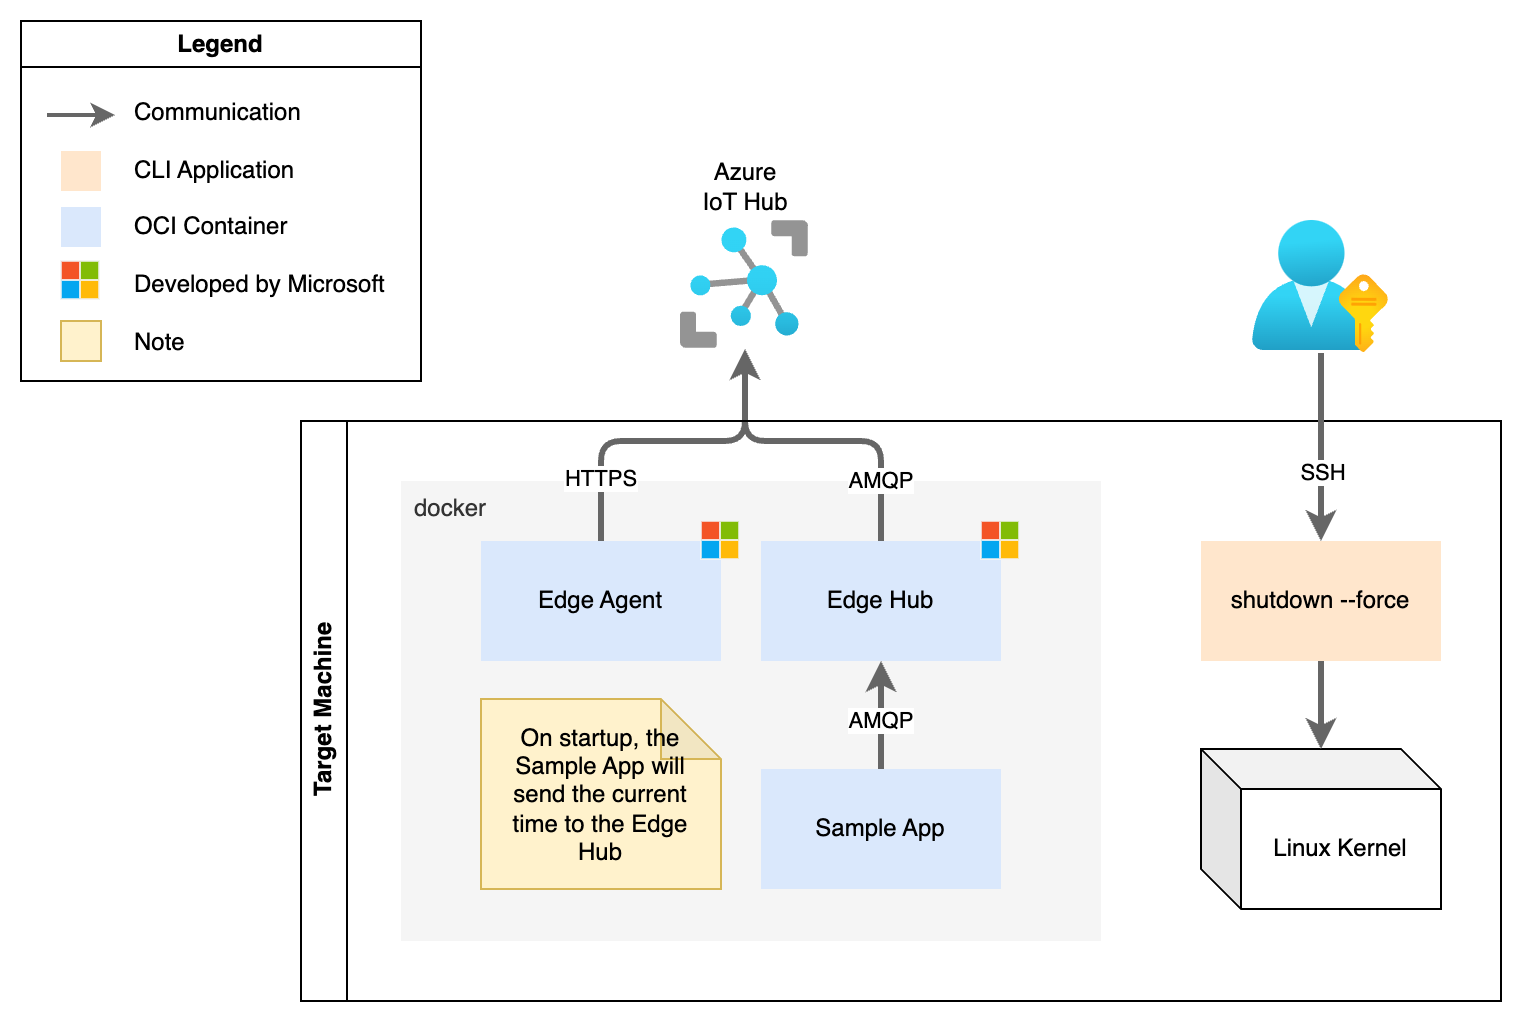
\includegraphics[width=0.75\textwidth]{fig/reboot-setup.drawio.png}
    \caption{Time To Recover Experiment Overview}
\end{figure}

\noindent
Just before the system is rebooted, the current time will be printed.
After the \ac{OS} rebooted and the Azure IoT Edge runtime has started, the
\textit{Edge Agent} container will send the current time to the Azure IoT Hub via
the Azure IoT Edge Hub, where it can be retrieved. The full shell command can
be seen in listing \ref{lst:reboot-command}.
\\

\begin{lstlisting}[
    caption=Shell Commands For Time To Recover Experiment,
    label=lst:reboot-command]
date +%s \
&& reboot
\end{lstlisting}

\noindent
When comparing the first timestamp ($t_0$) from the shell command output with the second
timestamp ($t_1$) from the \textit{Azure IoT Hub}, the time to recover can be calculated
as the delta between those two timestamps:

\begin{equation}
    T := |t_1 - t_0|
\end{equation}
However, since rebooting the \ac{OS} is a process with many variances, the experiment
must be repeated multiple times. If the experiment can be repeated $n$ times, where
$T_i$ represents the result of the $i$-th repetition, a mean value for $T$ can be
calculated as:

\begin{equation}
    \mu := \frac{\sum_{i=1}^{n}T_i}{n}
\end{equation}

\noindent
And the standard deviation for $T$ as:

\begin{equation}
   \sigma := \sqrt{\frac{\sum_{i=1}^{n}((T_i - \mu)^2}{n}}
\end{equation}

\noindent
Finally, the standard error for $T$ as:

\begin{equation}
    s := \frac{\sigma}{\sqrt{n}}
\end{equation}

\noindent
This experiment must be repeated until the standard error is low enough
to have a confident mean value for each \ac{OS}.

\subsection{Hypothesis}
The hypothesis is that the time to recover will be very similar for all
\ac{OS}s. Since they all run \textit{Linux}, the Azure IoT Edge runtime and
a similar set of software, such as \textit{systemd}, and \ac{SSH}. However, due
to the reduced size of \textit{reUpNix}, there may be a slight advantage in the
time to recover, since the \ac{OS} has to load less data from the disk. Further,
\textit{reUpNix} has a minified kernel and a reduced set of kernel modules.

\section{Container Updates}
\label{sec:container-updates}
When using Azure IoT Edge, \ac{IoT} applications are deployed as containers and
they tend change more frequent than the entire \ac{OS}. When a module is updated
with a new deployment manifest, Azure IoT Edge retrieves any new container
images that are not present on the device. It uses a \ac{UDS} to communicate
with the container runtime and instructs it to pull the image. The same can be
manually achieved with the \code{docker pull} command, when using \textit{Docker}
as the container runtime. Any container images which are already present on the
system will not be transmitted again.

In an scenario, where network connectivity is limited or expensive,
it should be avoided to pull the entire container image when only a few files have
changed. Since the \textit{Nix store} has a pretty efficient mechanism for
deduplicating files, it has to be investigated if \textit{reUpNix}'s
update mechanism can be used to update containers in a more efficient way.

The proposed approach is to pull and unpack the container images and their layers
during the build
process of the \ac{OS}, and then storing the resulting files in the
\textit{Nix store}. When a container image needs to be updated, it can
be included in the system configuration and updated with \textit{reUpNix}.
Since the container image layers are stored in the \textit{Nix store}, if an
image layer is already present, it will not be transmitted again. This is due
to the differential update mechanism of \textit{reUpNix}.
On boot, the container images can be loaded from the \textit{Nix store} and
loaded wit the \code{docker image load} command.

It needs to be verified by comparing the \textit{reUpNix} update size to the size
of the container layers,
which are updated by a docker pull, that this approach reduces the data transmitted.

\subsection{Hypothesis}
The hypothesis is that updating containers with \textit{reUpNix}'s differential
update mechanism will be more efficient than updating them with Azure IoT Edge or
the \code{docker pull} command. This is due to the fact, that if the
layers of the container image are extracted into the \textit{Nix store} and
updated with \textit{reUpNix}, a layer which is already present on the system
will not be transmitted again. This is very similar to how \code{docker pull}
works, but with the added benefit that the differential update is done on a
file level, so there is a potential for even more efficient updates. For example,
if a layer is updated which only contains minimal changes (e.g. only a few
changed files), the differential update will only transmit the changed files in
that layer instead of the entire layer.
